\chapter{Experiments}\label{Experiment}

To validate the feasibility and performance of VigiDroid as a practical on-device malware detection system, we constructed an experimental pipeline that couples traditional offline classification metrics with live hardware metrology collected from physical Android devices. Unlike evaluations that report accuracy only on desktop workstations, our methodology treats per-stage CPU time, memory delta, and battery consumption as first-class outcomes alongside F1-score and ROC-AUC.

This chapter details dataset provenance, split policies, feature engineering, ONNX deployment, the device evaluation APK set, the metrics conversion pipeline, and a comparative analysis explaining why different models achieve different results.

\section{Dataset Provenance and Characterization}

A foundational challenge in Android malware detection is temporal decay: models trained on historical samples often degrade when confronted with newer APKs whose authors exploit recently introduced APIs or obfuscation tricks. To mitigate optimistic bias, we evaluate VigiDroid using a strict chronological split rather than randomized $K$-fold cross-validation.

The experimental corpus comprises \textbf{13,528} APKs collected from AndroZoo~\cite{androzoo} and the public Hugging Face \texttt{android-apks} dataset~\cite{androidapks}, spanning 2020 through 2023 and labelled benign or malware according to the parent directory convention. The corpus occupies approximately 500\,GB on disk and is indexed uniformly across all model pipelines.

Two operational splits are used:
\begin{itemize}
 \item \textbf{In-sample training (2020--2021):} Used for feature discovery, MLDP permission selection, vocabulary construction, normalization statistics, and model training. For permission-centric models (LinRegDroid, MLDP-pruned), this period is further divided into 70\%/15\%/15\% train/validation/dev-test strata.
 \item \textbf{Out-of-sample temporal holdout (2022--2023):} Completely isolated during training. Models in the BM1/Pattern~A/cascade family evaluate on all 1,528 holdout APKs. Broadcast, XGBoost, ByteCNN, and fusion models use a 50/50 stratified partition of the holdout into validation ($n{=}764$) and test ($n{=}764$) subsets with seed~42.
\end{itemize}

\textbf{Important:} Metrics in Table~\ref{tab:results} must be read with the sample-size column in mind. Comparing a model scored on $n{=}1{,}528$ directly against one scored on $n{=}764$ without acknowledging the split difference would be misleading. We report both values faithfully and interpret them in Section~\ref{sec:results-analysis}.

\section{Feature Engineering, Extraction, and Normalization}

The extraction layer ingests multi-source characteristics directly from compressed APK archives without invoking heavyweight decompilers such as Apktool. Five standalone feature domains and several fusion combinations are supported.

\subsection{Manifest Permissions and Intents}
Using \texttt{pyaxmlparser} in the Python pipeline (and a native AXML decoder in Java), we isolate permissions and intent filters from binary \texttt{AndroidManifest.xml}. Strings are stripped of the \texttt{android.permission.} prefix, lower-cased, and mapped to a frozen vocabulary built on the training split. The result is a fixed-width binary presence--absence vector.

\subsection{Statically Registered Broadcast Receivers}
Following Mohsen and Ismail~\cite{broadcast}, we enumerate \texttt{<receiver>} elements and collect their \texttt{<intent-filter>} action strings (e.g., \texttt{BOOT\_COMPLETED}, \texttt{SMS\_RECEIVED}). These actions form an independent 70-dimensional feature block in the Broadcast+MLDP hybrid and Dex+Broadcast fusion models.

\subsection{DEX Header Metadata}
Instead of disassembling bytecode, we read bytes~8--111 of each \texttt{classes*.dex} file---a fixed 104-byte region encoding structural counts (methods, strings, type IDs, field references). Train-only min--max normalization is applied per byte offset, and multidex APKs are aggregated by sum-pooling (Algorithm~\ref{alg:dexheader}).

\subsection{Raw Tail Byte Sequences}
For domain-agnostic analysis, the last $N{=}1{,}024$ bytes of the raw APK archive are read without decompression. Tail bytes capture ZIP central-directory structures and attacker-appended payloads that header-only models may miss~\cite{byteCNN}.

\subsection{MLDP Permission Subsets}
On the training split only, the MLDP pipeline (Algorithm~\ref{alg:mldp}) selects a compact permission set~$S$ ($|S|{\leq}40$). This set is frozen and shipped inside each export bundle; the on-device extractor must not recompute it at runtime.

\section{Model Training and ONNX Export}

Models span three families: linear/statistical baselines (LinRegDroid MLR), ensemble trees (XGBoost on 2,500-d manifest OR vectors), and neural architectures (MLPs, ASCNN, 1-D CNN). Training hyperparameters are model-specific: BM1 uses SGD with learning rate 0.005 for 50 epochs; Pattern~A trains for 80 epochs; several hybrid models used abbreviated ``quick train'' schedules (1--3 epochs) during integration testing---a limitation noted in our results interpretation.

Every finalized PyTorch or scikit-learn model passes through the export pipeline shown in Figure~\ref{fig:onnx-deployment-pipeline}. The ONNX graph is verified against the source model on parity samples (Algorithm~\ref{alg:parity}) before staging to Android assets.

\begin{figure}[h]
\centering
\begin{tikzpicture}[
    node distance=1.25cm,
    block/.style={rectangle, draw, rounded corners, thick, minimum width=6.2cm, minimum height=0.85cm, align=center},
    note/.style={align=center, font=\small},
    arrow/.style={-{Stealth[length=3mm]}, thick}
]
\node[block] (trainingtools) {PyTorch / Scikit-Learn / XGBoost};
\node[block, below=of trainingtools] (weights) {Optimal Saved Weights};
\node[block, below=of weights] (onnx) {Standardized \texttt{.onnx} Binary};
\node[block, below=of onnx] (runtime) {On-Device Execution via ONNX Runtime};

\draw[arrow] (trainingtools) -- node[right, note] {Offline Training \& Validation} (weights);
\draw[arrow] (weights) -- node[right, note] {ONNX Operator Mapping (opset 14)} (onnx);
\draw[arrow] (onnx) -- node[right, note] {P8 Parity + Asset Staging} (runtime);
\end{tikzpicture}
\caption{Model optimization and ONNX deployment pipeline.}
\label{fig:onnx-deployment-pipeline}
\end{figure}

\section{Evaluation APK Set and On-Device Protocol}

No full APK corpus is stored in the git repository; evaluation relies on manifests and selectively staged binaries.

\subsection{Device Evaluation Manifest}
The primary on-device test set is defined in \texttt{Android\_Works/device\_eval\_manifest.csv}: all 1,528 temporal-holdout APKs renamed as \texttt{scan\_XXXX\_\{benign|malware\}.apk} and pushed to \texttt{/sdcard/Download/Scanable/} on the test phone (POCO F3). The manifest summary reports 1,050 benign and 478 malware samples totalling 22.31\,GB, distributed across size buckets from under 1\,MB to over 100\,MB.

\subsection{Parity and Regression Fixtures}
Each export bundle includes $\sim$10 parity samples with frozen input tensors and \texttt{expected\_prob.json}. Instrumented tests (\texttt{*ParityTest.java}, \texttt{*A4ParityTest.java}) run on bundled parity APKs in \texttt{androidTest/assets/}. A single known-malware fixture (\texttt{scan\_1514\_malware.apk}) validates that all eleven legacy stages complete successfully (P1 exit gate: 11/11 stages OK).

\subsection{Scan Phases}
Device evaluation proceeds in two phases orchestrated by \texttt{run\_phase3\_device\_scan\_a.sh} and \texttt{run\_phase4\_device\_scan\_b.sh}:
\begin{itemize}
 \item \textbf{Scan A:} Per-model isolated runs measuring parse, vectorize, inference, and total stage milliseconds.
 \item \textbf{Scan B:} Full cascade runs recording tier reached, models executed, models skipped, and exit reason.
\end{itemize}

\section{On-Device Hardware Profiling Infrastructure}

Figure~\ref{fig:on-device-hardware-profiling-workflow} traces the runtime path from UI trigger to metrics persistence. \texttt{ScanService.onHandleWork} opens a \texttt{FeatureContext} stream on each APK, delegates to \texttt{ScanOrchestrator}, and assembles per-stage telemetry through \texttt{ScanMetricsAssembler}.

\begin{figure}[h]
\centering
\begin{tikzpicture}[
    node distance=1.05cm,
    block/.style={rectangle, draw, rounded corners, thick, minimum width=5.4cm, minimum height=0.75cm, align=center, font=\small},
    tier/.style={rectangle, draw, thick, minimum width=6.4cm, minimum height=0.65cm, align=left, font=\small},
    side/.style={rectangle, draw, rounded corners, thick, minimum width=3.3cm, minimum height=0.65cm, align=center, font=\small},
    arrow/.style={-{Stealth[length=3mm]}, thick}
]
\node[block] (mainactivity) {MainActivity.startScan()};
\node[block, below=of mainactivity] (scanservice) {ScanService.onHandleWork()};
\node[block, below=of scanservice] (featurecontext) {FeatureContext.open(apk)};
\node[block, below=of featurecontext] (orchestrator) {ScanOrchestrator.run(ctx)};
\node[tier, below=0.7cm of orchestrator] (tierone) {Tier 1: MLDP-pruned \& Broadcast+MLDP};
\node[tier, below=0.75cm of tierone] (tiertwo) {Tier 2: MLDP+DEX cascade Mode B};
\node[tier, below=0.75cm of tiertwo] (tierthree) {Tier 3: Early-fusion ASCNN \& XGBoost};
\node[tier, below=0.75cm of tierthree] (tierfour) {Tier 4: ByteCNN fusion fallback};
\node[block, below=0.7cm of tierfour] (metrics) {ScanMetricsAssembler.toScanMetrics()};
\node[side, right=1.2cm of metrics] (capture) {CPU, RAM, Latency};
\node[block, below=of metrics] (writer) {MetricsWriter.appendScanJsonl()};
\node[side, right=1.2cm of writer] (save) {Local JSONL archive};
\node[block, below=of writer] (broadcast) {LocalBroadcast SCAN\_RESULT};
\node[side, right=1.2cm of broadcast] (ui) {Updates MainActivity UI};

\draw[arrow] (mainactivity) -- (scanservice);
\draw[arrow] (scanservice) -- (featurecontext);
\draw[arrow] (featurecontext) -- (orchestrator);
\draw[arrow] (orchestrator) -- node[right, font=\small] {Cascade gating} (tierone);
\draw[arrow] (tierfour) -- (metrics);
\draw[arrow] (metrics) -- (writer);
\draw[arrow] (writer) -- (broadcast);
\draw[arrow] (metrics) -- (capture);
\draw[arrow] (writer) -- (save);
\draw[arrow] (broadcast) -- (ui);
\end{tikzpicture}
\caption{On-device hardware profiling workflow.}
\label{fig:on-device-hardware-profiling-workflow}
\end{figure}

Each scan record captures: device metadata; APK name, path, SHA-256, and size; per-stage \texttt{parse\_ms}, \texttt{vectorize\_ms}, \texttt{inference\_ms}, \texttt{cpu\_ms}, \texttt{score}, and optional \texttt{stage1\_score}/\texttt{stage2\_score} for cascade models; cascade policy name, tier reached, exit reason, and models run/skipped; and session totals for wall time, CPU, PSS memory, dex count, and battery percentage change.

\section{Metrics Export and Conversion Pipeline}
\label{sec:metrics-pipeline}

On-device scans append one JSON object per line to \texttt{all\_scan\_metrics.jsonl} under the app's external files directory. For analysis compatibility with earlier tooling, we consolidate this append-only log into a legacy aggregate file \texttt{all\_scan\_metrics.json} using Algorithm~\ref{alg:jsonl} (implemented in \texttt{Shared\_pipeline\_Files/tools/jsonl\_to\_json.py}).

The broader plotting pipeline proceeds as follows:
\begin{enumerate}
 \item \textbf{Pull:} \texttt{pull\_device\_metrics.sh} retrieves JSONL from the device via ADB.
 \item \textbf{Fold:} \texttt{jsonl\_to\_json.py} merges scan and session records into \texttt{\{device, scans[], sessions[]\}}.
 \item \textbf{Validate:} \texttt{validate\_scan\_a.py} and \texttt{validate\_scan\_b.py} check schema completeness and cascade fields.
 \item \textbf{Aggregate:} \texttt{aggregate\_plot\_metrics.py} joins offline \texttt{test\_results.json} metrics with Scan~A/B device medians into \texttt{plot\_metrics\_table.json}, computing derived fields:
   \begin{equation}
     \mathrm{cost\_score} = \mathrm{stage\_total\_ms} + 10 \times \mathrm{mem\_mb}
   \end{equation}
   \begin{equation}
     \mathrm{composite} = 0.45 \times \mathrm{quality\_norm} + 0.30 \times \mathrm{tier\_weight} + 0.25 \times (1 - \mathrm{cost\_norm})
   \end{equation}
   where $\mathrm{quality\_norm}$ is the mean of accuracy, F1, and ROC-AUC normalized across models.
 \item \textbf{Plot:} \texttt{run\_all\_thesis\_plots.sh} generates publication-quality PNG figures (accuracy--latency scatter, inference breakdown, cascade exit tiers) under \texttt{Shared\_pipeline\_Files/results/figures/templates/}. Figures~\ref{fig:f1-cpu-scatter}--\ref{fig:cascade-exit} in this chapter provide TikZ equivalents for standalone PDF compilation.
\end{enumerate}

This pipeline is what produced the resource columns in Table~\ref{tab:results}: CPU and wall-time figures are medians from Scan~A on the POCO F3, not synthetic estimates.

\section{Results and Comparative Analysis}
\label{sec:results-analysis}

Table~\ref{tab:results} presents the unified offline--on-device comparison. External baselines (DroidCat, SeqMobile) are included for context; they were not re-implemented in VigiDroid but represent published upper bounds from dynamic and sequence-based approaches.

\begin{table}[H]
\label{tab:results}
\centering
\scriptsize
\setlength{\tabcolsep}{5pt}
\begin{tabular}{@{}l p{2.6cm} c c c c c c c c@{}}
\toprule
\textbf{Model} & \textbf{Features} & \textbf{$n$} & \textbf{Acc.} & \textbf{F1} & \textbf{AUC} & \textbf{CPU} & \textbf{Mem.} & \textbf{Time} & \textbf{Feasible} \\
\midrule
XGBoost & Manifest OR 2500-d & 764 & 0.937 & 0.888 & 0.991 & 97.4 ms & 0.02 MB & 100 ms & low \\
1D-CNN & Last 1024 bytes & 764 & 0.901 & 0.849 & 0.959 & 1.7 ms & 0.01 MB & 1.7 ms & low \\
MLP-H (BM1) & DEX header & 1528 & 0.967 & 0.944 & 0.968 & 0.7 ms & 0.01 MB & 0.4 ms & high \\
Early-Fusion ASCNN & Header + BoW & 1528 & 0.961 & 0.936 & 0.983 & 7.8 ms & 0.03 MB & 7.9 ms & medium \\
Dual-Branch & Header $\|$ BoW & --- & --- & --- & --- & 7.9 ms & 0.02 MB & 7.9 ms & medium \\
LinRegDroid & Permission flags & 1528 & 0.855 & 0.709 & 0.732 & 1.0 ms & 0.00 MB & 0.7 ms & low \\
MLDP-pruned & MLDP permissions & 1528 & 0.914 & 0.844 & 0.902 & 0.6 ms & 0.00 MB & 0.4 ms & medium \\
Broadcast+MLDP & Perms + receivers & 764 & 0.924 & 0.863 & 0.923 & 1.1 ms & 0.00 MB & 0.4 ms & medium \\
MLDP+DEX Cascade B & Perms $\rightarrow$ header & 1528 & 0.962 & 0.938 & 0.947 & 0.8 ms & 0.01 MB & 0.4 ms & high \\
Dex+Broadcast Fusion & Header + receivers & 764 & 0.970 & 0.950 & 0.979 & 0.9 ms & 0.01 MB & 0.5 ms & high \\
DroidCat & Dynamic analysis & --- & 0.974 & 0.978 & 0.98 & --- & --- & --- & --- \\
SeqMobile & Manifest + DEX seq. & --- & 0.977 & 0.977 & --- & --- & --- & --- & --- \\
\bottomrule
\end{tabular}
\caption{Offline accuracy metrics merged with on-device resource medians (POCO F3, Scan A). $n$ denotes temporal test set size; ``---'' indicates missing or stale offline run.}
\end{table}

\subsection{Visual Summary of Results}
Figures~\ref{fig:f1-cpu-scatter}--\ref{fig:cascade-exit} complement Table~\ref{tab:results} by exposing the accuracy--cost frontier and cascade efficiency visually.

\begin{figure}[H]
\centering
\begin{tikzpicture}[
  scale=0.92,
  font=\small,
  dot/.style={circle, fill=black!70, inner sep=1.8pt},
  lbl/.style={font=\scriptsize, align=left}
]
% axes
\draw[->, thick] (0,0) -- (11,0) node[right] {CPU time (ms, log scale)};
\draw[->, thick] (0,0) -- (0,6.2) node[above] {F1-score};
\foreach \x/\xl in {0/0.1, 1.7/1, 7.8/8, 97.4/100} {
  \pgfmathsetmacro{\px}{ln(\x+0.3)/ln(100)*10}
  \draw (\px,0.08) -- (\px,-0.08) node[below, font=\tiny] {\xl};
}
\foreach \y/\yl in {0/0.70, 2.5/0.75, 5/0.80, 7.5/0.85, 10/0.90, 12.5/0.95} {
  \draw (0.08,\y/2) -- (-0.08,\y/2) node[left, font=\tiny] {\yl};
}
% plot helper: x = ln(cpu+0.3)/ln(100)*10, y = f1*10/0.8 - 7
\node[dot] at (0.15,1.2) {};
\node[lbl, above right] at (0.15,1.2) {MLDP-pruned};
\node[dot] at (0.35,1.0) {};
\node[lbl, above right] at (0.35,1.0) {Broadcast+MLDP};
\node[dot] at (0.45,2.8) {};
\node[lbl, above right] at (0.45,2.8) {Cascade B};
\node[dot] at (0.5,3.5) {};
\node[lbl, above right] at (0.5,3.5) {Dex+Brdcst};
\node[dot] at (0.55,3.2) {};
\node[lbl, above right] at (0.55,3.2) {MLP-H};
\node[dot] at (2.8,1.8) {};
\node[lbl, above right] at (2.8,1.8) {Early-Fusion};
\node[dot] at (10,2.2) {};
\node[lbl, above left] at (10,2.2) {XGBoost};
% frontier hint
\draw[dashed, black!40] (0.2,1.0) .. controls (2,2.5) and (6,3.0) .. (10,2.2);
\node[font=\tiny\itshape, black!50] at (5.5,4.8) {Pareto frontier region};
\end{tikzpicture}
\caption{F1-score versus on-device CPU time (log-scaled horizontal axis). Dex+Broadcast fusion and MLP-H occupy the favourable upper-left region; XGBoost offers high separability at substantially higher cost.}
\label{fig:f1-cpu-scatter}
\end{figure}

\begin{figure}[H]
\centering
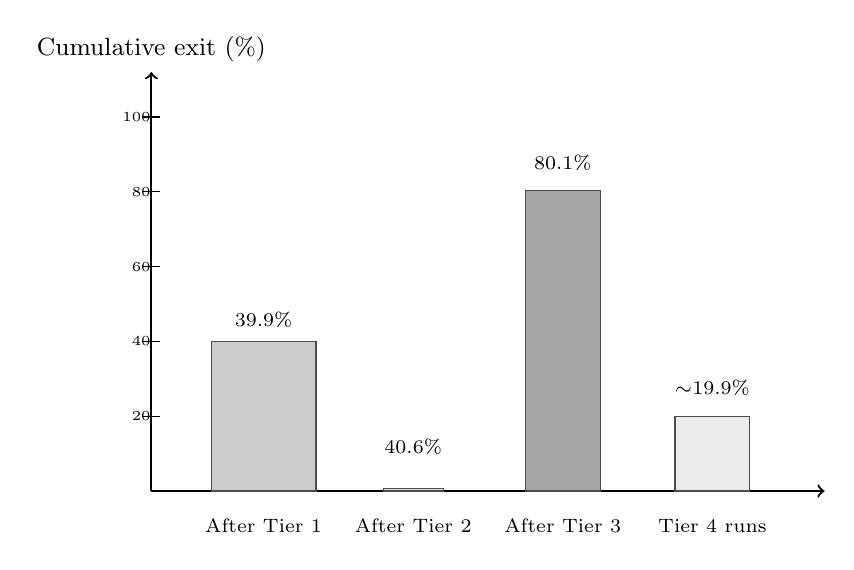
\begin{tikzpicture}[scale=0.95, font=\small]
% cumulative exit bars (scale: 1 unit = 20%)
\draw[->, thick] (0,0) -- (0,5.6) node[above] {Cumulative exit (\%)};
\draw[->, thick] (0,0) -- (9,0);
\foreach \y/\yl in {1/20, 2/40, 3/60, 4/80, 5/100} {
  \draw (-0.12,\y) -- (0.12,\y) node[left, font=\tiny] {\yl};
}
% Tier checkpoints (x positions 1.5, 3.5, 5.5, 7.5)
\fill[black!20, draw=black!70] (0.8,0) rectangle (2.2,1.996); % 39.9%
\node[below, font=\scriptsize] at (1.5,-0.25) {After Tier 1};
\node[above, font=\scriptsize] at (1.5,2.05) {39.9\%};
\fill[black!12, draw=black!70] (3.1,0) rectangle (3.9,0.028); % +0.7%
\node[below, font=\scriptsize] at (3.5,-0.25) {After Tier 2};
\node[above, font=\scriptsize] at (3.5,0.35) {40.6\%};
\fill[black!35, draw=black!70] (5.0,0) rectangle (6.0,4.02); % 80.1%
\node[below, font=\scriptsize] at (5.5,-0.25) {After Tier 3};
\node[above, font=\scriptsize] at (5.5,4.15) {80.1\%};
\fill[black!8, draw=black!70] (7.0,0) rectangle (8.0,1.0); % remaining to 100%
\node[below, font=\scriptsize] at (7.5,-0.25) {Tier 4 runs};
\node[above, font=\scriptsize] at (7.5,1.15) {$\sim$19.9\%};
\end{tikzpicture}
\caption{Cascade cumulative early-exit rates on 764 validation APKs (\texttt{cascade\_policy.json}). More than 80\% of samples are resolved before the ByteCNN backstop.}
\label{fig:cascade-exit}
\end{figure}

\begin{figure}[H]
\centering
\resizebox{0.88\columnwidth}{!}{%
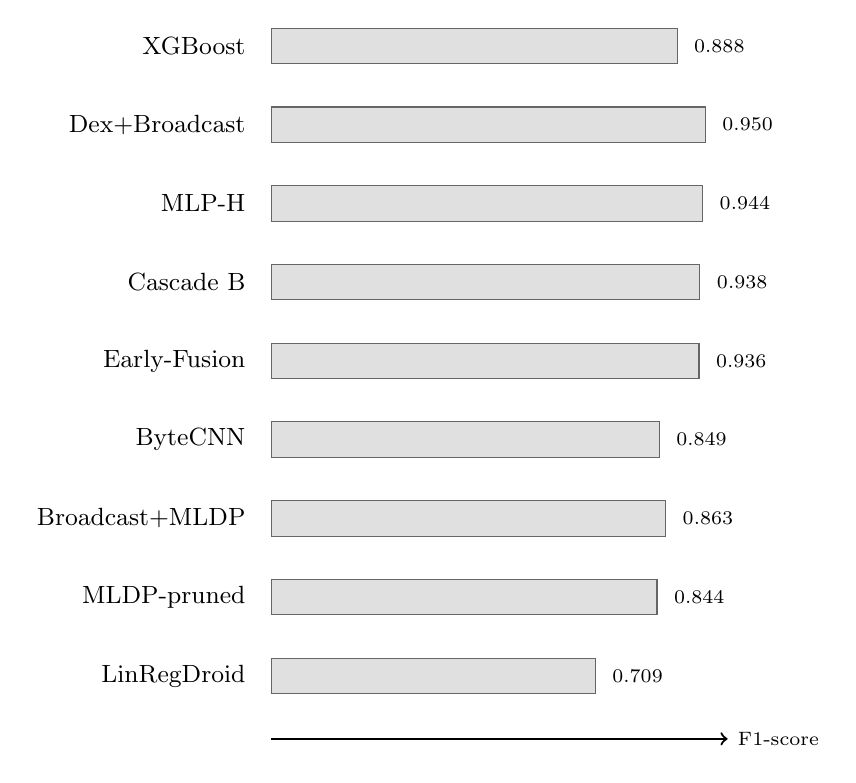
\begin{tikzpicture}[font=\small, bar/.style={rectangle, draw=black!60, fill=black!12, minimum height=0.45cm}]
\def\barwidth{5.8}
% horizontal bars: label, f1, width factor
\foreach \y/\name/\fval in {
  0/LinRegDroid/0.709,
  1/MLDP-pruned/0.844,
  2/Broadcast+MLDP/0.863,
  3/ByteCNN/0.849,
  4/Early-Fusion/0.936,
  5/Cascade B/0.938,
  6/MLP-H/0.944,
  7/Dex+Broadcast/0.950,
  8/XGBoost/0.888
} {
  \node[anchor=east] at (-0.2, \y) {\name};
  \pgfmathsetmacro{\bw}{\fval*\barwidth}
  \node[bar, minimum width=\bw cm, anchor=west] at (0,\y) {};
  \node[anchor=west, font=\scriptsize] at (\bw+0.1,\y) {\fval};
}
\draw[->, thick] (0,-0.8) -- (\barwidth,-0.8) node[right, font=\scriptsize] {F1-score};
\end{tikzpicture}%
}
\caption{Offline F1-score ranking of implemented models (temporal test splits as in Table~\ref{tab:results}).}
\label{fig:f1-ranking}
\end{figure}

\subsection{Why Models Differ: A Feature--Capacity--Cost Lens}
The spread in Table~\ref{tab:results} is not noise; it reflects deliberate trade-offs among feature expressiveness, model capacity, training convergence, and extraction cost.

\paragraph{Permission-only models (LinRegDroid, MLDP-pruned).}
LinRegDroid uses the full 173-permission vocabulary with a linear decision boundary. It is extremely fast but caps out at F1~0.709 because many malware families declare innocuous permission sets while hiding behaviour in bytecode or native code. MLDP-pruned improves to F1~0.844 by discarding irrelevant permissions and emphasising malware-associated combinations, yet it still cannot see structural dex anomalies.

\paragraph{Broadcast-enhanced models (Broadcast+MLDP, Dex+Broadcast fusion).}
Adding receiver actions provides a second manifest signal orthogonal to permissions: persistence hooks (\texttt{BOOT\_COMPLETED}) and SMS interception (\texttt{SMS\_RECEIVED}) are rare in benign utilities but common in trojans. Dex+Broadcast fusion reaches the highest accuracy among our deployed models (97.0\%, F1~0.950) because it combines this manifest signal with bytecode structural counts from the dex header---capturing both \emph{when} and \emph{how much} code is present.

\paragraph{DEX header models (BM1, cascades, early fusion).}
The 104-byte header encodes complexity metrics cheaply. BM1 alone achieves F1~0.944, rivalling far heavier pipelines. Early-fusion ASCNN adds a 4,381-dimensional manifest bag-of-words, lifting AUC to 0.983 but increasing vectorization cost to $\sim$8\,ms. The MLDP+DEX cascade Mode~B matches BM1 accuracy (F1~0.938 end-to-end) while skipping dex reads whenever stage-one permissions are decisive---the best accuracy--cost compromise in the production cascade.

\paragraph{Heavy models (XGBoost, ByteCNN).}
XGBoost achieves the highest AUC (0.991) by OR-ing thousands of manifest and API tokens across all dex files, but its $\sim$100\,ms inference makes it suitable only as a Tier~3 specialist. ByteCNN captures tail-byte patterns invisible to structural parsers; it is expressive but trained on $n{=}764$ and used as a Tier~4 backstop rather than a first-line screen.

\paragraph{Dual-Branch (Pattern B).}
The dual-branch ASCNN architecture was implemented but not fully trained in this workspace; device assets may be stale. We report its resource profile from staged exports but omit offline accuracy until a complete P1--P8 run is finished.

\subsection{Cascade Efficiency}
Calibration on 764 validation APKs shows Tier~1 early exit in $\sim$39.9\% of cases, rising to $\sim$80.1\% cumulative exit before Tier~4. This means the expensive XGBoost and ByteCNN stages execute on fewer than one in five APKs during normal cascade operation---a direct battery-saving consequence of the tiered design.

\subsection{Comparison with External Baselines}
DroidCat and SeqMobile report higher F1-scores (0.978 and 0.977 respectively) but rely on dynamic analysis or full API-call sequencing with multi-second latencies on flagship hardware. VigiDroid's Dex+Broadcast fusion closes much of this gap (F1~0.950) at sub-millisecond cost, supporting our thesis that carefully chosen static shortcuts can approach dynamic accuracy without execution overhead.

\endinput
